\section{RASimAs}


\subsection{Herramienta \acs{ITGVPH}}
\label{result:herramienta}

En el primer caso de uso que se presenta, la herramienta \ac{TPTVPH} permite modificar un modelo de paciente virtual de una postura original a la posición requerida previamente a su incorporación en un simulador. Esta herramienta es flexible y robusta ante modelos incompletos o del que no se dispongan sus propiedades mecánicas. 

Con el objetivo los usuarios puedan entrenar con una variabilidad anatómica extensa, el proyecto \ac{RASimAs} ha propuesto la creación del entorno \ac{ITGVPH}. Esta \emph{suite} es el resultado de la integración de varias herramientas, en la cual, cada una de ellas trabajará de manera independiente. %Esta herramienta se encargará de generar una base de datos de pacientes virtuales que servirán como modelos de entrada para el simulador \ac{RASim}. 


Como se detalló en la sección \ref{rasim:herramienta}, el entorno \ac{ITGVPH} se compone de tres tareas:

\begin{itemize}
    \item El primer módulo de la herramienta es el encargado de hacer un registro entre imágenes de pacientes reales y el modelo \emph{ZygoteBody}$^{TM}$. De esta manera, se recupera información real para generar variabilidad anatómica. Este módulo ha sido descrito en \cite{deOliveira:2015}, desarrollado por \ac{UKA-IMI}. 
    \item En cuanto al módulo del posicionamiento de pacientes virtuales \ac{TPTVPH}, además de su presentación en el capítulo \ref{cap:posing}, se han obtenido durante el desarrollo de esta tesis las siguientes publicaciones \cite{ceig.20151197, SUJAR2018268}.
    \item
    El último componente es el encargado de la generación de un modelo biomecánico para el modelo de salida del paso anterior. Este módulo se ha desarrollado por \ac{INRIA}. Puede consultarse en \cite{ded3.3}.
\end{itemize}

Es importante mencionar, que el modelo virtual más utilizado para la realización de las pruebas de los distintos componentes era \emph{ZygoteBody}$^{TM}$. Este modelo presenta algunos problemas en sus representaciones superficiales como puede comprobar en \cite{zaitseva}. Aun así, la herramienta se ha diseñado para que pueda utilizarse cualquier modelo comercial.% que han derivado en la realización de algoritmos más robustos como se puede observar en la sección \ref{posing:result}.

Por último, esta herramienta ha sido evaluada por los supervisores asignados por la Unión Europea. En las distintas reuniones de seguimiento del proyecto, esta herramienta ha sido valorada positivamente debido a los resultados obtenidos.
\todo{incluyo algún documento oficial o algo? me comentaste que destacaron el trabajo que se realizó}




\subsection{RASim}
\label{result:rasim}

\todo{Marcos says:da  validez aparente al prototipo de RASim con trackers}
El objetivo del proyecto \ac{RASimAs} es la consecución de un entorno de entrenamiento de \ac{RA} que permita mejorar la efectividad y la tasa de éxito del procedimiento.  En esta sección, se analizará los resultados obtenidos del simulador \ac{RASim} donde se ha realizado las contribuciones técnicas de esta tesis.

Como se ha introducido en el capítulo \ref{rasim:rasim}, el simulador esta compuesto por distintos módulos software:

\begin{itemize}
    \item El \emph{renderizado} de la escena virtual utilizando \emph{H3D} \cite{sensegraphics2012open}.
    \item Para la simulación física y la respuesta háptica\cite{needleinsertion} se ha utilizado la librería \ac{SOFA} \cite{sofaweb}.
    \item El módulo encargado de la simulación de la adquisición de la imagen de \ac{US} \cite{Law2015}.
    \item El \ac{Courseware} gestiona y controla todos los módulos anteriores (ver sec. \ref{rasim:courseware}).
\end{itemize}


En relación al prototipo completo, los miembros médicos presentes en el proyecto \ac{RASimAs} (pertenecientes a la universidad de \emph{Cork}), han realizado una validación de contenido, sobre la guía citada en la sección \ref{art:ra}. En la figura \ref{fig:RAsteps}, se han identificado los pasos que el simulador \ac{RASim} es capaz de simular y puedan ser utilizado para el entrenamiento de anestesistas. %Estos pasos están basados en la guía que se utiliza en la educación de los estudiantes de la universidad de Cork.
%A continuación, se mostrará la lista de aquellos pasos que el simulador es capaz de simular para el entrenamiento de la \ac{RA}.


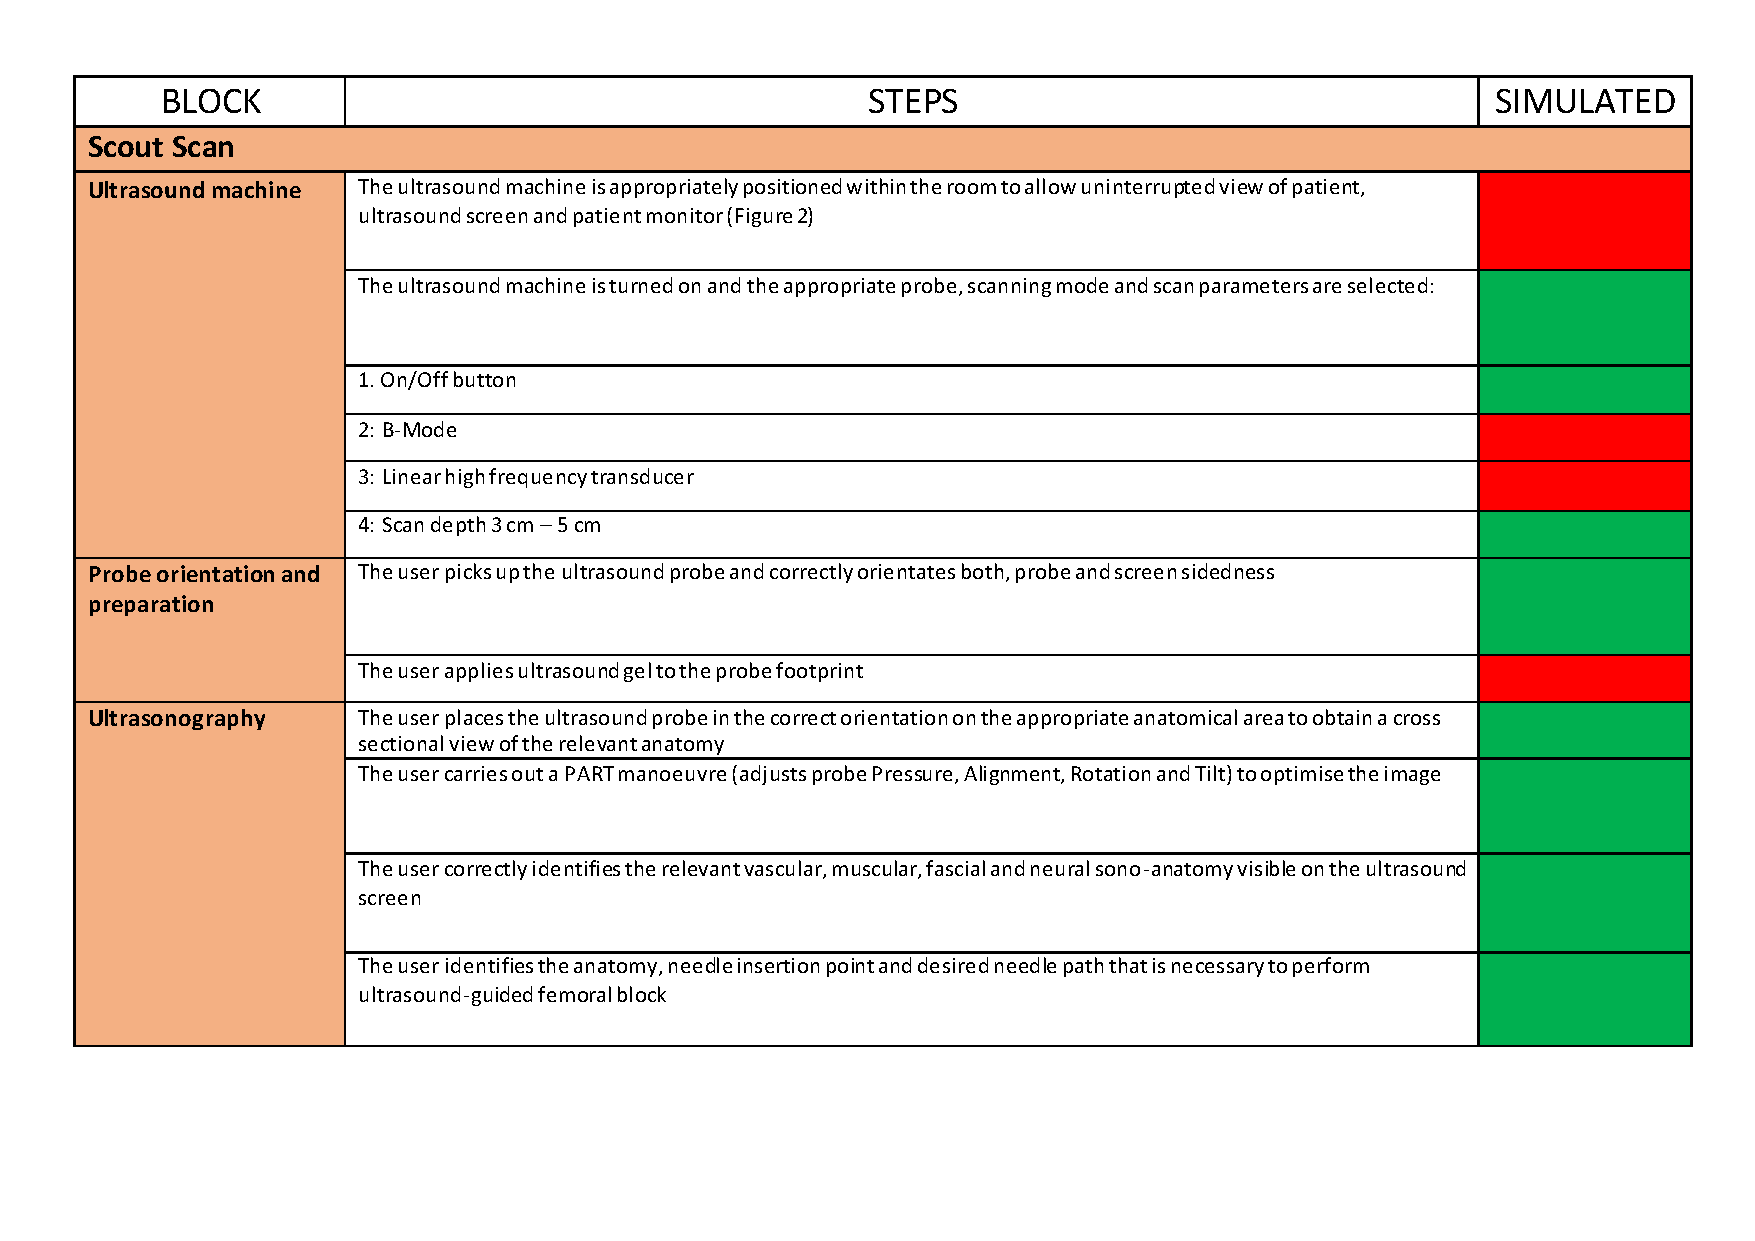
\includepdf[pages=1,frame,landscape]{PDFs/RA} 
\includepdf[pages=2,frame,landscape]{PDFs/RA}
\includepdf[pages=3,frame,landscape]{PDFs/RA}
\begin{figure}
    \centering
       \caption{Relación entre las etapas y fases del procedimiento de \ac{RA} y la funcionalidad del simulador \ac{RASim} }
    \label{fig:RAsteps}
\end{figure}

%\subsection{Rendimiento}
En términos computacionales, el sistema era capaz de satisfacer los requisitos de interactividad que se le presuponen a un simulador de \ac{RV} y exigidos por el propio proyecto. El simulador \ac{RASim} mostraba una ejecución interactiva en todas las etapas incluyendo aquellas computacionalmente más costosas. Por ejemplo, el sistema era capaz de responder ante la deformación de la anatomía por el contacto de la sonda de \ac{US} al apoyarse en el modelo virtual. Por otra parte, el sistema respondía con fluidez cuando el usuario introducía la aguja y se devolvía retroalimentación háptica a la vez que se seguía ejecutando la simulación de la imagen de \ac{US}. El usuario no percibía en ningún caso un retraso de las respuestas físicas o de las imágenes mostradas por los monitores.

En las presentaciones previas del prototipo, el comité médico del proyecto valoraba positivamente la deformación de los tejidos y la imagen resultante de \ac{US}. En cuanto a la respuesta háptica de la aguja, no se valoró positivamente por parte del comité, no siendo posible su evaluación clínica. Debido a problemas de precisión de los dispositivos hápticos (presentaban defectos de fábrica), los médicos consideraron que podría introducir sesgos en los aprendices. A partir de una propuesta de la \ac{URJC}, se procedió a sustituir los dispositivos hápticos por unos \acs{tracker}s magnéticos que permitió conseguir una evaluación favorable por parte de los evaluadores. Aunque, debido a estos problemas, no se pudo realizar una evaluación clínica antes de la finalización del proyecto.

%4clínica oportunas entre las que se propusieron: validez predictiva, de contenido y de constructo.





\subsection{Discusión}
\label{rasim:discusion}

%\ac{RASim} presenta una carencia fundamental  carencias frente al procedimiento de \ac{RA}. 
Como ha sido comentado anteriormente, el simulador \ac{RASim} presenta problemas con el dispositivo háptico. La respuesta física del movimiento de la aguja es un punto fundamental en el entrenamiento del procedimiento. Aunque este módulo ha sido validado correctamente fuera del simulador \cite{needleinsertion}, no ha sido posible su correcta validación en el prototipo \ac{RASim}.
%Por otra parte, en cuanto a la imagen de \ac{US}, la principal queja a la que se enfrenta el simulador es que proporciona una imagen, aunque parecida, demasiado clara y perfecta y no refleja completamente las dificultades que se presentan las imágenes ultrasónicas reales.

En primer lugar, es importante comentar el resultado final de la evaluación de la comisión europea sobre el proyecto \ac{RASimAs}. Este comité califico el proyecto con un \emph{progreso aceptable} debido a las dificultades para finalizar la evaluación clínica. Los problemas inesperados fueron los determinantes para que esta evaluación no pudiera hacerse en el tiempo esperado. Aun así, se valoró muy positivamente el módulo de \ac{RAAs} y el estado del prototipo final de \ac{RASim}. El propio comité animó a seguir con los trabajos necesarios que hagan falta para la finalización del \ac{RASim} y que pueda ser utilizado en entornos reales para el beneficio de los estudiantes de anestesiología.

Lamentablemente, la validación del simulador completo con la herramienta de aprendizaje no ha sido posible por numerosas dificultades.
Cuando se disponía ha realizarse la valoración previa del comité médico del proyecto \ac{RASimAs} en los centros de los distintos miembros, se descubrió que los prototipos habían sufrido daño en el transcurso de su transporte.% Los principales componentes del computador habían quedado inservibles, en concreto la \ac{GPU}. Estos desperfectos dieron lugar a replantear la planificación de las evaluaciones del prototipo.

En cuanto se pudo resolver este problema, se procedió a presentar los dispositivos al comité médico para comprobar y realizar una validación aparente. Por su parte, el comité expresó ciertas preocupaciones sobre la falta de correspondencia entre la posición del dispositivo y su representación virtual. Debido a que la falta de equivalencia entre la posición de la aguja y la sonda de \ac{US}, no era posible que el usuario obtuviera una imagen clara de la aguja en el procedimiento, y esto podría ocasionar malas prácticas en el desempeño de los futuros médicos. %Este fallo no se había producido en el desarrollo del prototipo y no estaba presente en los equipos de desarrollo. 

%Entre los participantes del desarrollo del prototipo se descubrió que los errores de precisión provenían de los dispositivos hápticos. Estos no proporcionaban una rotación adecuada según su posición real como se puede observar en la figura \ref{fig:errorhaptic}.
En las imágenes, se puede apreciar que la rotación del actuador no corresponde con los valores recogidos por el software, por lo tanto, no habría una correspondencia directa. Para ilustrar la desviación que causaban, se rotaba el dispositivo hasta el punto en el que marcaba una rotación simple de 90 grados, pero el actuador se encontraba más allá de la horizontal. Además, por cada dispositivo, el error era diferente, por lo cual no cabía la posibilidad de crear una solución única para todos los prototipos. También se podía inducir que el problema parecía ser de \emph{hardware} y no un error del \emph{software} del dispositivo.


\begin{figure}[h]
\centering
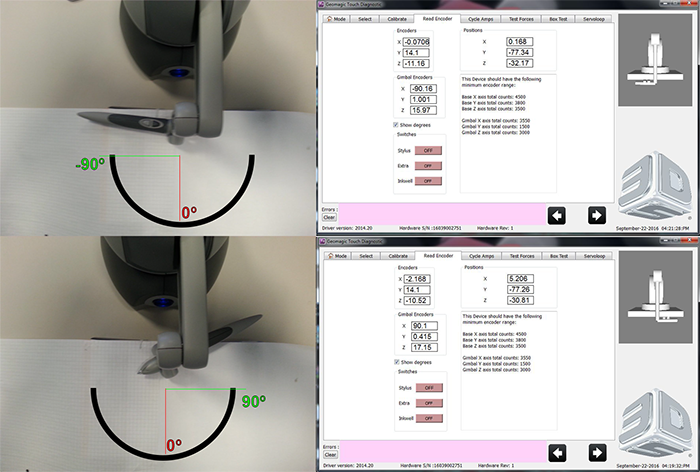
\includegraphics[width=0.9\linewidth]{IMG/errorhaptic.png}
\caption{\label{fig:errorhaptic}Diferencias de rotaciones reales frente a las proporcionadas por el dispositivo a través de su herramienta de calibración.}
\end{figure}

%Con la esperanza de una solución, se contactó con la empresa que ha distribuido los dispositivos. La empresa detectó este mismo error en los dispositivos de nueva facturación y comunicó que propondrían una solución para ello. Esta solución no ha llegado en un tiempo razonable en la que permitiera proceder a la evaluación del prototipo en un entorno clínico. A su vez, 
Se propusieron alternativas para los dispositivos, como por ejemplo utilizar solo \ac{tracker}s sacrificando la retroalimentación háptica, la cual era un punto fundamental del proyecto. Debido a la conclusión del proyecto y, por tanto, la falta de recursos económicos no se ha podido completar ninguna alternativa en el tiempo necesario para realizar una validación en un entorno clínico.



%Por último, hay que tener en cuenta que ciertos aspectos protocolarios del procedimiento no están incluidos en el simulador, como tampoco se encuentra la simulación de las tareas de la técnica aséptica.




